\chapter{Sistemas de vapor}

Fuentes utilizadas:
\begin{itemize}
	\item \citetitle{molanes2009vapor} de \cite{molanes2009vapor}
	\item \citetitle{sarco-distribucion} de \cite{sarco-distribucion}
\end{itemize}

Los sistemas de vapor son utilizados para transportar energía calorífica desde su generación hasta los puntos de consumo. Constan de tres partes principales: la generación en la caldera, el circuito de vapor propiamente dicho y el circuito de condensado.



\section{Pipping}

\subsection{Materiales utilizados}
\begin{itemize}
    \item Ferrosos: Aceros al carbono Aleaciones Acero inoxidable
    \item No ferrosos: Cobre Latón Bronces Metal Monel
    \item Plásticos: PVC, teflón, poliestireno, polietileno
    \item Otros: cerámica, vidrios, hormigón, porcelana.
\end{itemize}

\subsection{Caños y tubos}

La diferencia principal entre caños y tubos radica en cómo se define el diámetro nominal. En el caso de los caños, el diámetro nominal coincide con el diámetro exterior solo a partir de tamaños de 14''. En cambio, en los tubos, el diámetro nominal coincide con el diámetro exterior o interior, dependiendo de las especificaciones del fabricante.


   \subsection{Dimensionamiento y selección}
Para dimensionar las tuberías, es necesario determinar tanto el diámetro como el espesor. Ambos valores están estandarizados, aunque el espesor se especifica mediante el denominado Schedule, que define una serie de espesores normalizados según el diámetro nominal.
    \subsubsection{Cálculo del diámetro}
    % Se calculan según una fórmula que relaciona la resistencia del material, los diámetros, el espesor, la presión interna a la que está sometido y factores de soldadura y corrosión.
    % Los métodos de cálculo son:\begin{itemize}
    %     \item Según fórmula código ASME: se calcula la presión de trabajo admisible adoptando un schedule y verificando que sea superior a la presión de trabajo
    %     \item Según fórmula Schedule.
    %     \item Cálculo simplificado: se adopta un schedule y se verifica la presión admisible frente a la de trabajo.
    %     \item Por gráficas o tablas
    % \end{itemize}


    Para hallar el diámetro de la tubería existen dos métodos: en función de la velocidad de trabajo, y en función de la presión. Al aplicar un método, se deben verificar los valores con el otro.
    \begin{itemize}
        \item \textbf{La velocidad del fluido}\\
        Para tuberías de distribución de vapor saturado seco, las velocidades máximas razonables suelen estar entre 25 y 40 m/s —deben considerarse como el máximo ya que para velocidades mayores aparecen el ruido y la erosión—. En líneas de gran longitud, las velocidades se limitan a 15 m/s para evitar grandes caídas de presión.


        Una vez \emph{adoptada la velocidad}, el diámetro puede calcularse por \emph{método gráfico} o \emph{analítico}.
        
        Para el \textbf{método gráfico}, se utiliza el ábaco mostrado en la \autoref{fig:abaco-velocidad} \parencite[pág. 16]{sarco-distribucion}, que permite obtener el diámetro de la tubería a partir de los siguientes datos: presión del vapor, temperatura (en caso de vapor recalentado), caudal y velocidad.
        
        El \textbf{método analítico} consiste en calcular el tamaño de tubería como: \(\dot{V}=A \cdot v\) donde $V$ es el caudal volumétrico, $A$ la sección transversal de la tubería, y $v$ la velocidad adoptada. A partir de esta expresión se puede calcular el área y, por ende, el diámetro de la tubería.

        \begin{figure}[H]
            \centering
            \caption{Gráfico para dimensionar tuberías de vapor (método de la velocidad).}\label{fig:abaco-velocidad}
            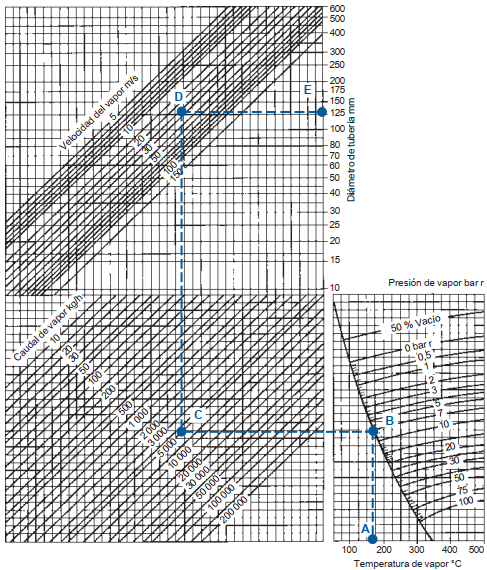
\includegraphics[width=.7\linewidth]{vapor/tabla-velocidad}
        \end{figure}
        
        \item \textbf{La caída de presión} 
        
        Este método es apropiado cuando las caídas de presiones resulten críticas o de mayor interés. Se deben conocer las presiones de suministro y consumo. Este método es más frecuentemente utilizado en el dimensionamiento de líneas más largas y de mayor diámetro. Entre los métodos más conocidos se utilizan los dos siguientes: \emph{método gráfico} y método de los \emph{factores de presión}.
        
        El \textbf{método gráfico} es más rápido y se hace uso del ábaco de la \autoref{fig:abaco-presion} \parencite[pág. 17]{sarco-distribucion} si se conocen las siguientes variables: temperatura del vapor, presión, caudal y caída de presión. Para líneas largas, el ábaco empleado es el de la \autoref{fig:abaco-presion-largas} que tiene un cuenta la longitud \parencite[pág. 18]{sarco-distribucion}.

        Para aplicar el \textbf{método de factores de presión} se aplican los siguientes pasos:
        \begin{enumerate}
            \item Longitud equivalente total (L)
            
            Se calcula sumando la longitud física de la tubería y una longitud adicional que representa la resistencia de los accesorios (codos, válvulas, etc.), basándose en la experiencia (ej. 10\% o 20\% de la longitud física).
            
            \item Caudal total de vapor
            
            Se suman el caudal de vapor requerido y el caudal de vapor que se condensa debido a las pérdidas de calor en la tubería (se considera 1\% cada 30m para tubería aislada).
            
            \item Factores de presión (P1 y P2)
            
            Se obtienen los factores de presión correspondientes a la presión inicial y final según la Tabla 8 de la guía \parencite[pág. 57]{sarco-distribucion}.
            
            \item Cálculo del Factor F
            
            La fórmula es: $F = \dfrac{P1 - P2}{L}$.
            
            \item Selección del tamaño de tubería
            
            Usando el factor F, se busca en la Tabla 9. Se selecciona el tamaño de tubería cuyo factor 'x' (capacidad en kg/h) sea igual o superior al caudal total de vapor calculado.
            
            \item Ajuste del Factor F
            
            
            
            \item Verificación de velocidad
            
            Se usa el factor 'y' de la Tabla 9 y el volumen específico del vapor (Tabla 8) para calcular la velocidad real. Este método de dimensionado a menudo resulta en velocidades inferiores a las máximas permitidas por velocidad, ya que prioriza la limitación de la caída de presión.
        \end{enumerate}
         \begin{figure}[H]
            \centering
            \caption{Gráfico para dimensionar tuberías de vapor (método de la presión).} \label{fig:abaco-presion}
            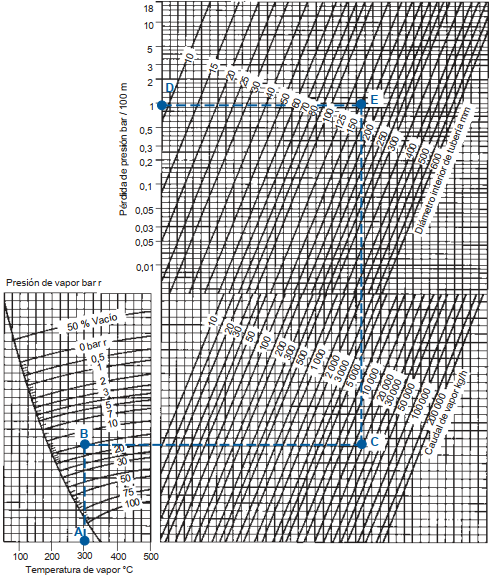
\includegraphics[width=.7\linewidth]{vapor/tabla-presion}
        \end{figure}
         \begin{figure}[H]
            \centering
            \caption{Gráfico para dimensionar tuberías de gran longitud (método de la presión).} \label{fig:abaco-presion-largas}
            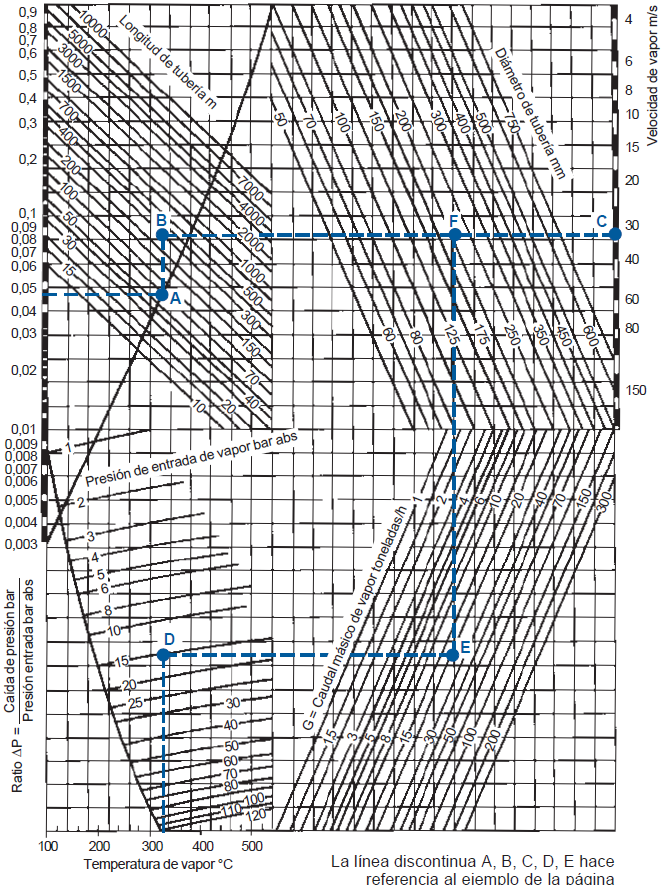
\includegraphics[width=.7\linewidth]{vapor/abaco-presion-largas}
        \end{figure}
    \end{itemize}
    
    \textbf{Sobredimensionar} implica mayor coste, más condensado por pérdidas de calor y peor calidad de vapor en los puntos de consumo o requerimientos más elevados en las calderas. \textbf{Subdimensionar} provoca alta velocidad y caída de presión, suministro insuficiente de vapor, mayor riesgo de erosión, golpe de ariete y ruidos. 
    
    \subsubsection{Schedule}
    Es un número adimensional que indica el espesor del tubo o caño de forma aproximada. Están tabulados en las normas ANSI.
    \[SH=1000\dfrac{P_i}{\sigma_{adm}}\]

\subsection{Líneas de distribución y condensado}
\subsubsection{Línea de distribución}
    El vapor generado en la caldera debe ser conducido a través de las tuberías hasta el punto en que se requiere esta energía calorífica. Inicialmente habrá una o más tuberías principales que transporten el vapor de la caldera en la dirección de la planta de utilización del vapor. 

    Las tuberías deben montarse con una pendiente descendente (mínimo 40 mm cada 10 m) en la dirección del flujo para que el condensado y el vapor vayan juntos. 
    


\subsubsection{Línea de condensado}
    El agua que se utiliza en las calderas, que posteriormente será vapor para distintos puntos de consumo, es agua tratada, por lo que es muy valiosa y resulta importante considerar en el diseño el retorno de condensado siempre que resulte factible.
    
    En la puesta en marcha, la cantidad de condensado será mayor debido a que el vapor se utiliza para calentar tanto las tuberías de distribución como los equipos en los puntos de consumo.

\subsubsection{Puntos de purga} Se deben instalar puntos de purga en los puntos bajos del sistema. En líneas largas, se necesitan puntos de purga cada 30-50 m, además de en los puntos bajos.
    
    
    Se debe usar un pozo de goteo (T) en tramos rectos para recoger el condensado que fluye a gran velocidad. La boca del purgador se eleva ligeramente para evitar suciedad. Los pozos de goteo grandes ayudan a albergar condensado durante la puesta en marcha hasta que la presión es suficiente para purgar.
    \begin{figure}[h]
        \centering
        \caption{Punto de purga para una línea de condensado.}
        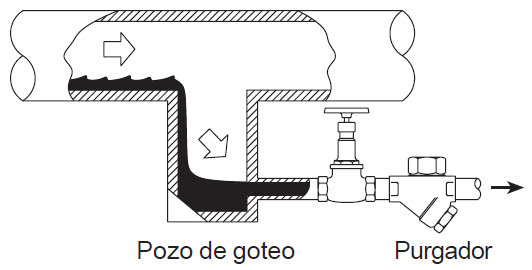
\includegraphics[width=0.5\linewidth]{vapor/punto-de-purga.png}
    \end{figure}

\subsubsection{Golpe de ariete} Se da cuando el condensado golpea contra las tuberías o accesorios, provocando daños o elevadas presiones. Se puede evitar asegurando que el condensado no se acumule. 


Las fuentes comunes de golpe de ariete incluyen pandeos en la línea, uso incorrecto de reductores/filtros y purga inadecuada.
    
    \subsubsection{Derivaciones}
     Las conexiones de derivación deben tomar el vapor de la parte superior de la tubería principal para obtener vapor más seco. Se necesita un punto de purga en los puntos bajos de las derivaciones.

    \begin{figure}
        \centering
        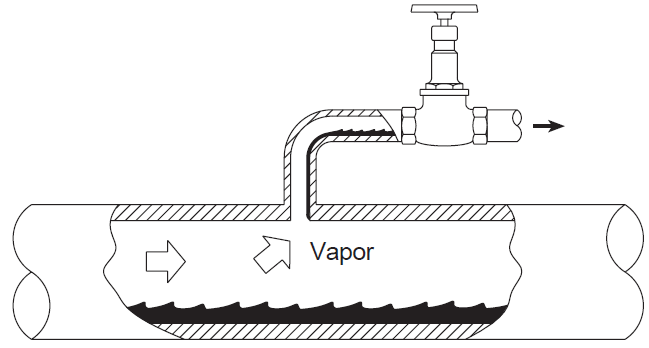
\includegraphics[width=0.5\linewidth]{vapor/conexion-derivacion.png}
        \caption{Punto de conexión para derivación.}
        \label{fig:conexion-derivacion}
    \end{figure}

     La válvula de la \autoref{fig:conexion-derivacion} debe instalarse lo más próximo a la toma para evitar que el condensado se deposite en ese ramal si existen paradas muy largas.\\

     Por otro lado, en los puntos de consumo (extremos de las derivaciones) también deben instalarse puntos de purga ya que también hay puntos bajos (\autoref{fig:derivacion-purga}). Lo más común es un punto de purga cerca de una válvula de aislamiento o una válvula de control.
     
    \begin{figure}
        \centering
        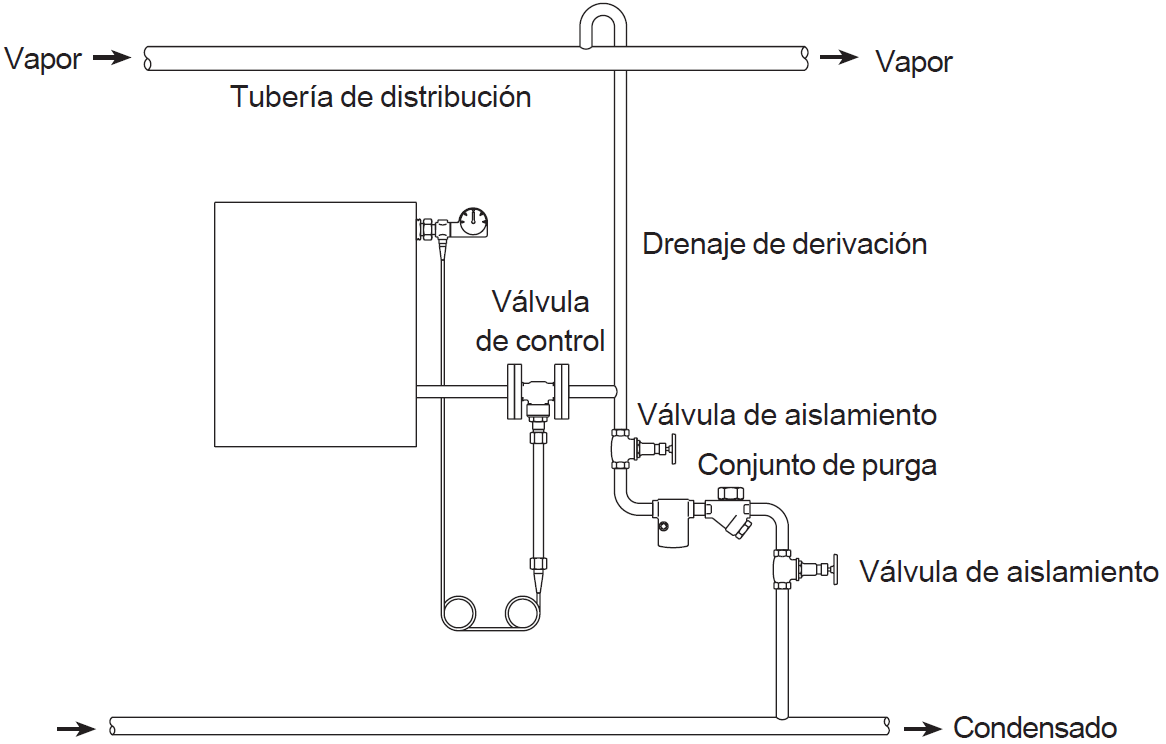
\includegraphics[width=0.5\linewidth]{vapor/derivacion-purga.png}
        \caption{Punto de conexión para derivación.}
        \label{fig:derivacion-purga}
    \end{figure}
\subsubsection{Eliminación de aire}   
El aire y otros gases no condensables entran en el sistema y se acumulan. El aire reduce la transferencia de calor significativamente y puede reducir la temperatura del vapor, afectando el proceso. También contribuye a la corrosión. Los eliminadores de aire automáticos —que no son más que purgadores de vapor termostáticos— son esenciales para una rápida puesta en marcha y mantener la eficiencia.

\section{Dilatación y soportes}

La tubería debe tener suficiente flexibilidad para poder adaptarse a los movimientos causados por el calentamiento y la dilatación. Esta flexibilidad puede ser inherente al propio diseño de la tubería si tiene longitudes razonables y suficientes curvas.


Una consideración particular es la diferencia de dilatación entre una línea de vapor caliente y una línea de retorno de condensado que discurre paralela a una temperatura más baja. Esta diferencia de movimiento relativo requiere que la conexión del purgador a la línea de retorno tenga suficiente flexibilidad para evitar tensiones excesivas en el ramal.

\subsection{Soportes}
\begin{itemize}
    \item Los soportes son necesarios para sostener el peso de la tubería y su contenido.
    \item La frecuencia y el tipo de soportes varían según el diámetro de la tubería, el material (acero o cobre) y si la tubería está en posición horizontal o vertical.
    \item Los soportes deben estar diseñados específicamente para adaptarse al diámetro exterior de la tubería; no es recomendable usar soportes sobredimensionados.
    \item Es preferible montar los soportes en las uniones de las tuberías (curvas, 'T', válvulas, bridas) para eliminar las tensiones en las juntas roscadas o bridadas.
    \item Además de en las uniones, los soportes deben instalarse a intervalos regulares que no superen ciertas distancias recomendadas según el material y la posición (horizontal o vertical) de la tubería. Se utiliza una tabla con distancias recomendadas entre soportes para tuberías de acero suave y cobre de diferentes diámetros nominales \parencite[pág. 42]{sarco-distribucion}.
    \begin{figure}[H]
        \centering
        \caption{Intervalo recomendado entre soportes para tuberías.}
        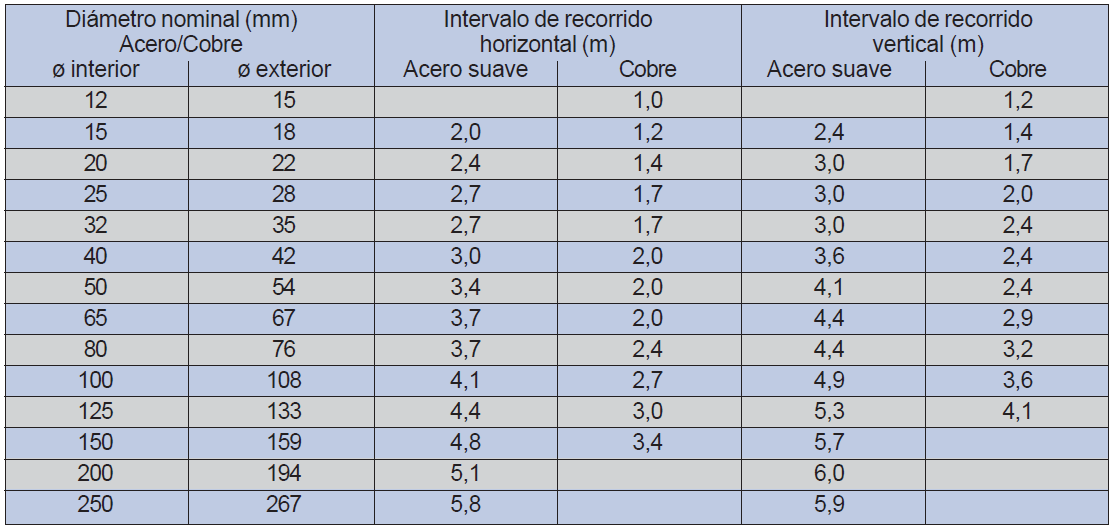
\includegraphics[width=0.8\linewidth]{vapor/soportes.png}
    \end{figure}
\end{itemize}

\subsection{Accesorios de dilatación}
Cuando la flexibilidad natural de la tubería no es suficiente para absorber la dilatación, se emplean accesorios diseñados específicamente para este fin, que se montan en línea y acomodan la expansión sin cambiar la longitud total de la tubería.
\begin{itemize}
    \item \textbf{Curva completa}, \textbf{Lira} o herradura, y \textbf{Curvas de dilatación}: Estos accesorios aprovechan la flexibilidad del propio material de la tubería al estar conformado en curvas. Se recomienda montarlos horizontalmente para evitar la acumulación de condensado; si se montan verticalmente, se requiere un punto de purga antes del accesorio. Las curvas de dilatación pueden fabricarse con tramos rectos y codos soldados.
    \item \textbf{Junta deslizante}: Se usan por su reducido espacio. Requieren un anclaje y guiado muy rígidos para contrarrestar la fuerza que la presión interna ejerce sobre el casquillo. Si no está bien alineada, el casquillo puede curvarse, y requiere mantenimiento regular del prensaestopas.
    \item \textbf{Fuelles}: Se montan en línea y no necesitan empaquetadura. Similar a la junta deslizante, la presión interna tiende a alargarlos, por lo que necesitan anclajes y guías robustos. Existen diseños de fuelles que pueden absorber movimiento axial, lateral y angular. La instalación debe seguir siempre las instrucciones del fabricante.
\end{itemize}

\section{Reductores de presión}
Distribuir a alta presión permite tuberías de menor diámetro, reduce pérdidas de calor y costes, produce vapor más seco y mejora la capacidad de la caldera para manejar fluctuaciones de carga. Si se distribuye a alta presión, se requiere reducción de presión en el punto de utilización.


El método más común para reducir la presión son los reductores de presión o \emph{cuadros de regulación}. Un reductor de presión se compone de:
\begin{itemize}
    \item Separador de gotas (1): evacua la humedad del vapor, impurezas y condensado, hacia el purgador. Su selección se basa en gráficos de dimensionado que consideran presión, caudal, tamaño y caída de presión.
    \item Filtro (3): retiene partículas de impurezas que podrían dañar a elementos como purgadores, válvulas, medidores, etc. Deben montarse delante de estos elementos. Para evitar el golpe de ariete en los filtros, cuando forman parte de una línea de vapor, deben montarse con la cesta en posición horizontal.
    \item Válvulas reguladoras (2)
    \item Manómetros (4)
    \item Válvula reductora (5)
    \item Válvula de seguridad (6)
    \item Conjunto de purga para el condensado. Se compone de \begin{itemize}
        \item Válvulas de cierre (7): para aislar la sección del circuito en caso de mantenimiento
        \item Filtro (8)
        \item Purgadores o trampas de vapor (9).
        \item Válvula de retención (10): para que no retorne el condensado durante las paradas.
    \end{itemize}
    
\end{itemize}

\begin{figure}[H]
    \centering
    \caption{Cuadro de regulación extraído del trabajo práctico hecho.}
    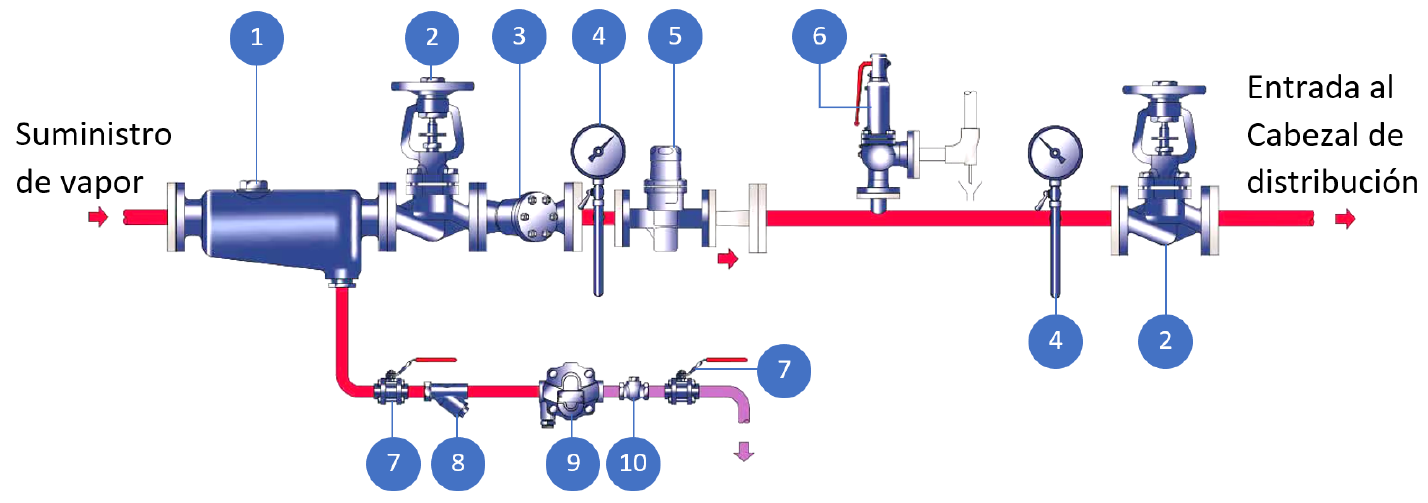
\includegraphics[width=0.8\linewidth]{vapor/regulador.png}
\end{figure}

\section{Separador de gotas}

        Un separador de gotas evacuará tanto las gotitas de agua de las paredes de la tubería como la humedad suspendida en el vapor. La presencia y efecto del golpe de ariete puede erradicarse montando un separador en la tubería principal de vapor y con frecuencia será una alternativa más económica que alterar la tubería para vencer este fenómeno.

        Para su selección se debe tener en cuenta la presión interior, el caudal de vapor y la velocidad del flujo. Se hace uso del ábaco de la \autoref{fig:tabla-seleccion-separador} \parencite[pág. 26]{sarco-distribucion}. La zona sombreada indica el rango de funcionamiento óptimo, donde el separador operará cerca del 100\% de rendimiento.

        % \textbf{Ejemplo de selección}:

        % Determinar el tamaño de un separador para un caudal de 500 kg/h a una presión de 13 bar.
        % \begin{figure}[H]
        %     \centering
        %     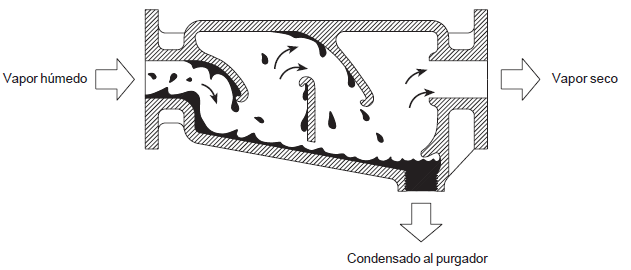
\includegraphics[width=0.5\linewidth]{vapor/separador-gotas.png}
        %     \caption{Separador de gotas}
        %     \label{fig:separador-gotas}
        % \end{figure}
        
        % \begin{enumerate}
        %     \item Trace una línea que una la presión con el caudal. A-B
        %     \item  Trace la línea horizontal B-C
        %     \item Cualquier curva de separador que corta la línea B-C dentro del área sombreada operará cerca del 100 \% de rendimiento.
        %     \item Adicionalmente, la línea de velocidad para cualquier tamaño puede determinarse tranzando una línea vertical D-E (por ejemplo 18 m/s para una unidad DN32).
        %     \item Tambien puede determinarse la caída de presión tranzando las líneas E-F y A-F. El punto de intersección es la caída de presión a través del separador, en este caso es aproximadamente 0,037 bar.
        % \end{enumerate}
        
    \begin{figure}[H]
        \centering
        \caption{Tabla de selección del separador de gotas}
        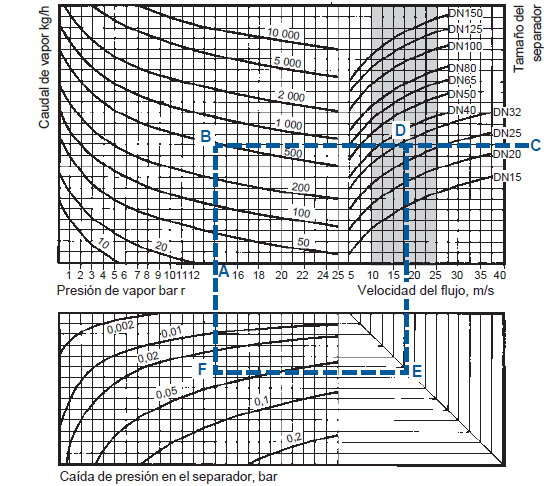
\includegraphics[width=.7\linewidth]{vapor/tabla-seleccion-separador.png}
        \label{fig:tabla-seleccion-separador}
    \end{figure}
    
\section{Purgadores}
Los purgadores, o también conocidos como trampas de vapor, tienen como objetivo descargar el condensado, aire y otros gases no condensables, sin permitir el escape de vapor vivo.

\begin{itemize}
    \item En la puesta en marcha el purgador debe ser capaz de descargar aire. Hasta que el aire sea desplazado, el vapor no puede entrar en su espacio propio y el calentamiento se hace lento. Utilizados con este propósito, en orden de efectividad, se encuentran los purgadores termostáticos, los purgadores de boya cerrada con eliminadores termostáticos incorporados, y por último, los purgadores termodinámicos.
    
    \item Una vez eliminado el aire, el purgador debe eliminar condensado pero no el vapor. Escapes de vapor en este punto implican un proceso poco eficiente. Así que el purgador ha de dejar pasar el condensado mientras que atrapa al vapor. Si la velocidad de traspaso de calor es crítica en el proceso, se ha de descargar el condensado inmediatamente y a la temperatura de vapor. 
\end{itemize}

Se clasifican en:\begin{itemize}
    \item Mecánicos
    \item Termostáticos
    \item Termodinámicos
\end{itemize}

\subsection{Selección de un purgador}

Se debe tener en cuenta parámetros como \begin{itemize}
    \item Presiones máximas de vapor y condensado
    \item Presiones de trabajo de vapor y condensado
    \item Temperaturas y caudales
    \item Si el proceso permite anegamiento
\end{itemize}

\subsection{Revaporizado}

Es el vapor flash generado por la disminución de presión del condensado en el purgador.

\subsection{Purgadores termostáticos}
Este tipo actúa por diferencia de temperatura. El purgador contiene un líquido con una temperatura de ebullición algo inferior a la del agua, entonces, cuando alcanza determinada temperatura, se expande y cierra la válvula. Por este motivo, el condensado debe enfriarse primero antes de ser descargado. Es muy útil en las condiciones frías del arranque, cuando la cápsula está en posición de reposo y la válvula está abierta, permitiendo la salida del aire libremente. 


Existen purgadores\begin{itemize}
    \item De expansión líquida:
    \item De presión equilibrada: La expansión de un líquido en una pequeña cápsula, actúa la válvula de cierre cuando detecta una temperatura cercana a la del vapor saturado. Resiste heladas y golpes de ariete.
    \item Bimetálico: La dilatación en un elemento bimetálico actúa la válvula de cierre cuando detecta una temperatura cercana a la del vapor saturado.
\end{itemize}

\begin{figure}[h]
    \centering
    \caption{Estados de un purgador de presión equilibrada.}
    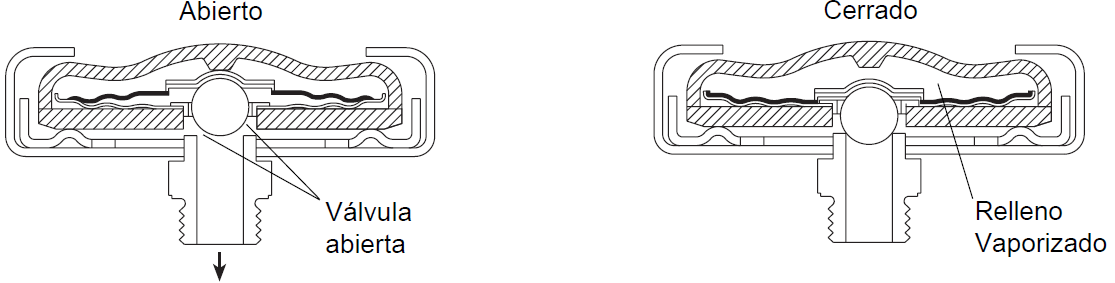
\includegraphics[width=0.75\linewidth]{vapor/purgador-presion-equilibrada.png}
\end{figure}

\begin{figure}[h]
  \centering
  \caption{Purgadores termostáticos.}
  \begin{subfigure}{0.45\textwidth}
    \caption{Purgador de presión equilibrada.}
    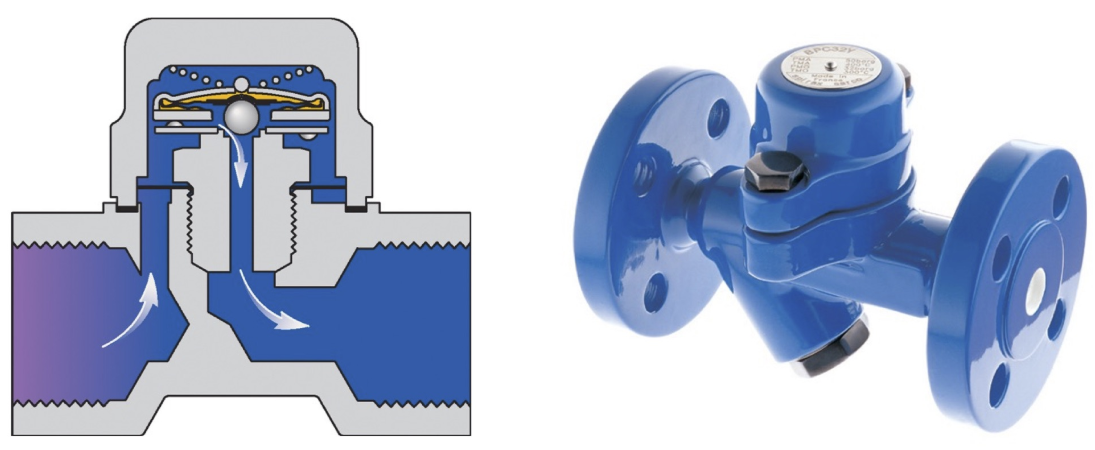
\includegraphics[width=\linewidth]{vapor/presion-equilibrada.png}
  \end{subfigure}
  \begin{subfigure}{0.45\textwidth}
    \caption{Purgador bimetálico.}
    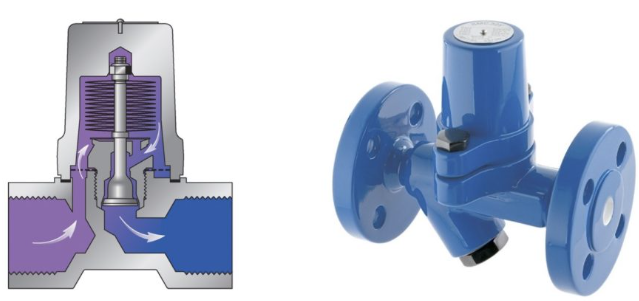
\includegraphics[width=\linewidth]{vapor/bimetalico.png}
  \end{subfigure}
\end{figure}


\subsection{Purgadores mecánicos}

\subsubsection{De boya o flotador}
Son purgadores de descarga continua. Se puede instalar una válvula tipo termostática para eliminar el aire desplazado en la marcha.

\subsubsection{De balde invertido}

\subsection{Purgadores termodinámicos}
: no tan utilizadas. Funcionan por diferencia de velocidades de condensado.

\section{Calderas}

\subsection{Tipos de calderas}
Las calderas se pueden clasificar según cómo se distribuye el agua en:
\begin{itemize}
    \item Humotubulares: el agua se encuentra en un tanque y se transforma en vapor debido a los gases calientes que circulan en tubos. Son tanques sometidos a presión.
    \item Acuotubulares: el agua que se transforma en vapor circula a través de tubos verticales. Son de mayor tamaño que las anteriores.
\end{itemize}

\subsection{Selección}

\begin{itemize}
    \item Caudal de vapor: el requerido, más el perdido en el condensado, más previsión de ampliación.
    \item Presión de trabajo: debe contemplar la mayor presión requerida de los puntos de utilización, la caída de presión y las pérdidas de calor en las tuberías.
\end{itemize}
